\chapter{Framework di Anonimizzazione}

\nt{Molti di questi Framework sono superati, ai giorni nostri \fancyglitter{differential privacy} ha soppiantato tutti gli altri.}

\section{Il Problema dell'Anonimità}

\paragraph{Problema:}

\begin{itemize}
  \item Molte agenzie, istituzioni, organizzazioni, etc. rendono pubblicamente disponibili dati sensibili riguardanti persone: 
    \begin{itemize}
      \item Molti microdata per le analisi. 
      \item Spesso la legge richiede la loro anonimizzazione.
    \end{itemize}
  \item I microdata vengono \fancyglitter{sanificati} (rimossi gli id espliciti). 
  \item Non è sufficiente per preservare la privacy:
    \begin{itemize}
      \item Suscettibili a \fancyglitter{linking attack}. 
      \item Databases pubblici possono rilevare identità "segrete".
    \end{itemize}
\end{itemize}

\subsection{Linking Attack}

Nel 2001, Latanya Sweeney riuscì a reidentificare i record medico del governatore del Massachussetts: 
\begin{itemize}
  \item Il Massachussetts colleziona e pubblica dati medici sanificati per gli impiegati statali. 
  \item I dati dei votanti registrati sono pubblicamente disponibili.
\end{itemize}

\begin{figure}[h]
    \centering
    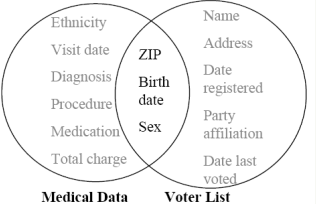
\includegraphics[scale=0.41]{03P/LA.png}
    \caption{Linking Attack del 2001.}
\end{figure}

\paragraph{Ruoli degli attributi nei microdata:}

\begin{itemize}
  \item Identificatori espliciti: sono rimossi. 
  \item Quasi identificatori: possono essere usati per reidentificare individui. 
  \item Attributi sensibili: portano informazioni sensibili.
\end{itemize}

\nt{Il goal della preservazione della privacy è quello di \fancyglitter{deassociare} individui da informazioni sensibili.}

\dfn{Quasi Identificatori (Tore Dalenius, 1986)}{
  I quasi identificatori sono attributi che non sono univoci di per sé, ma che se combinati con altri quasi identificatori possono creare un identificatore univoco. 
}

\paragraph{I quasi identificatori sono facilmente attaccabili:}

\begin{itemize}
  \item Linking attack di Sweeney. 
  \item Arvind Narayanan e Vitaly Shmatikov hanno usato i quasi identificatori per deanonimizzare dati di Netflix.
\end{itemize}

\section{K-Anonimity}

\dfn{Quasi Identificatori}{
  Assumiamo $A = {a_1,\dots,a_n}$ come insieme di $n$ attributi e $D$ un dataset definito su $A$. Un quasi identificatore di $D$ è un sottoinsieme di attributi $QI \subseteq S$ che deve essere controllato prima della pubblicazione.
}


\nt{Per risolvere il problema Sweeney e Samarati proposero, nel 1998, la \fancyglitter{k-anonimity}.}

\dfn{K-Anonimity}{
  Assumiamo $T$ come dataset su un insieme $A={a_1,\dots,a_n}$ di attributi e $QI_T$ come insieme di quasi identificatori di $T$. $T$ \textit{soddisfa} la k-anonimity se e solo se per ogni quasi identificatore $QI \in QI_T$ ogni sequenza esistente di valori attribuiti a $QI$ compare almeno con $k$ occorrenze in $T$.
}

\clm{}{}{
  Ogni pubblicazione dei dati deve essere controllata in modo che la combinazione dei valori dei quasi identificatori può essere associata ad almeno $k$ tuple:
\begin{itemize}
  \item Si nasconde ogni individuo in $k-1$ altri individui. 
  \item I linking attack non possono essere effettuati con una confidenza superiore a $\frac{1}{k}$.
\end{itemize}

}

\paragraph{Condizioni sufficienti per la k-anonimity:}

\begin{itemize}
  \item Ogni insieme di valori associati a un quasi identificatore deve avere almeno $k$ occorrenze. 
  \item Gli attributi sensibili non sono considerati.
\end{itemize}

\subsection{Come Ottenere la K-Anonimity?}

Esistono diversi modi per ottenere la k-anonimity:

\begin{itemize}
  \item \fancyglitter{Generalizzazione:} il valore di un dato attributo è rimpiazzato da uno più generale. 
    \begin{itemize}
      \item Negli ZIP code si nascondono le ultime due cifre $(10149 \rightarrow 101**, 10126 \rightarrow 101**)$. 
      \item La data di nascita rimpiazzata dall'anno di nascita $(27/09/1964 \rightarrow 1964, 30/09/1964 \rightarrow 1964)$.
    \end{itemize}
  \item \fancyglitter{Soppressione:} proteggere informazioni sensibili rimuovendole.
\end{itemize}

\begin{figure}[h]
    \centering
    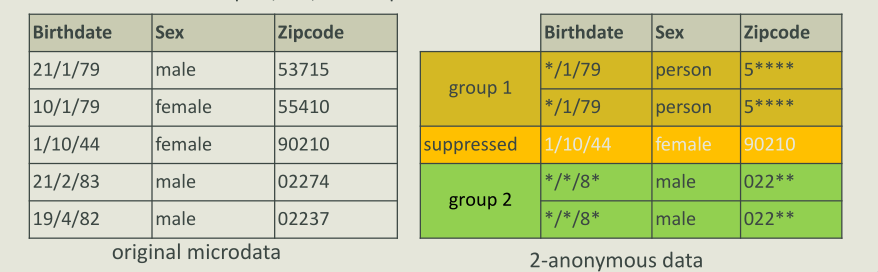
\includegraphics[scale=0.41]{03P/kanon.png}
    \caption{Esempio di applicazione di k-anonimity.}
\end{figure}

\paragraph{Privacy vs. Utility:}

\begin{itemize}
  \item Se i dati vengono troppo anonimizzati diventano inutili. 
  \item Per cui non si deve anonimizzare più del necessario.
\end{itemize}

\dfn{Domain Generalization Hierarchy}{
  Una gerarchia di generalizzazione su un dominio $(DGH_D)$ di un attributo $A$ è un ordine parziale su un insieme di domini $Dom_A = {D_0,\dots,D_n}$ che soddisfa le seguenti condizioni:
  \begin{itemize}
    \item Ogni dominio $D_i$ ha al più una generalizzazione diretta. 
    \item Tutti gli elementi massimi di $Dom$ sono singletons (per far sì che tutti i valori in ogni dominio possano essere generalizzati in un singolo valore).
  \end{itemize}
}

\clm{}{}{
Esempio: 
\begin{itemize}
  \item Z0: 53715, 53710, 53706, 53703. 
  \item Z1: 5371*, 5370*. 
  \item Z2: 537**.
\end{itemize}
}

\cor{Value Generalization Relationship}{
  Una relazione di valori generalizzati associa a ogni valore $v_i$ del dominio $D_i$ un valore univoco $v_j$ in un dominio $D_j$ dove $D_j$ è una diretta generalizzazione di $D_i$.
}

\nt{La relazioni implicano, per ogni dominio $D$, l'esistenza di un Value Generalization Relationship $VGH_D$. $VGH_D$ può essere rappresentato come un albero con il valore più generale come radice e i valori più specifici come foglie.}

\cor{Generalization Lattice}{
  Dato un dominio di tuple $DT = < D_{A1},\dots,D_{An}$ tale che $D_{Ai}$ sia in $Dom_{Ai}$, la gerarchia di generalizzazione del dominio di $DT$ è 

  $$DGH_{DT} = DGH_{D_{A1}} x \dots x DGH_{D_{An}}$$
 
  $DGH_{DT}$ definisce un reticolo il cui elemento minimo è $DT$.
}

\dfn{Generalized Table with Suppression}{
  Dato un insieme di attributi $A = {A_1,\dots,A_n}$ e due tabelle $T_i$ e $T_j$ definiti su $A$, la tabella $T_j$ è una generalizzazione della tabella $T_i$ ($T_i \leq T_j$) se e solo se: 
  \begin{itemize}
    \item Il dominio di ogni attributo $A_x$ in $T_j$ è uguale o una generalizzazione del dominio di $A_x$ in $T_i$. 
    \item Ogni tupla $t_j$ in $T_j$ ha una tupla $t_i$ corrispondente in $T_i$ tale che per ogni attributo $A_x$, $t_j[A_x]$ è uguale o una generalizzazione di $t_i[A_x]$.
  \end{itemize}
}

\nt{Non tutte le generalizzazioni hanno lo stesso valore.}

\cor{Vettore Distanza}{
  Date due tabelle $T_i$ e $T_j$ definite sullo stesso insieme di elementi $A = {A_1,\dots, A_n}$ tale che $T_i \leq T_j$, il vettore distanza di $T_j$ da $T_i$  è il vettore $DV_{ij} = [d_1,\dots,d_n]$ dove ogni $d_x$ è la lunghezza del percorso univoco tra $dom(A_x, T_i)$ e $dom(A_x, T_j)$ in $DGH_{DX}$.
}

\begin{figure}[h]
    \centering
    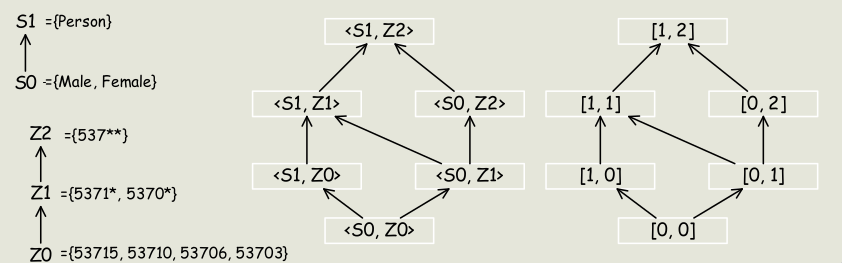
\includegraphics[scale=0.39]{03P/vd.png}
    \caption{Percorsi di generalizzazione.}
\end{figure}

\nt{L'obiettivo è  trovare la minima generalizzazione che soddisfi la k-anonimity. In questo modo si ha sia anonimizzazione che perdità di informazioni limitata (massimizzazione dell'utilità). Ciò si può fare trovando il vettore distanza minimo.}

\dfn{K-Minimal Generalization with Suppression}{
Date due tabelle $T_i$ e $T_j$ tali che $T_i \leq T_j$ e MaxSup lo specifico threshold di soppressione accettabile, $T_j$ è una generalizzazione k-minima di $T_i$ se e solo se: 
\begin{itemize}
  \item $T_j$ soddisfa la k-anonimity. 
  \item La soppressione è minimale. 
  \item $|T_j| - |T_i| \leq$ MaxSup. 
  \item $\forall T_x: T_i \leq T_x, T_x$ soddisfa gli altri tre punti $\Rightarrow DV_{ix} \geq DV_{ij}$.
\end{itemize}
}

\paragraph{Livelli di granularità delle tecniche di k-anonimity:}

\begin{itemize}
  \item Generalizzazione:
    \begin{itemize}
      \item Su singola colonna: passi di generalizzazione su tutti i valori di una colonna. 
      \item Su singola cella: per una specifica colonna. 
    \end{itemize}
  \item Soppressione: 
    \begin{itemize}
      \item Su singola riga: si sopprime tutta la tupla. 
      \item Su singola colonna: si oscurano tutti i valori di una colonna. 
      \item Su singola cella: solo alcune celle sono cancellate.
    \end{itemize}
\end{itemize}

\subsection{Algoritmi per la K-Anonimity}

Il problema di trovare le tabelle con la minima k-anonimity, con generalizzazione di attributi e soppressione di tuple, è \fancyglitter{NP-hard}. La grande maggioranza degli algoritmi proposti hanno un tempo computazionale esponenziale con il numero dei valori degli attributi (approccio greedy). Quando il numero $|QI|$ degli attributi nei quasi identificatori è piccolo rispetto al numero $n$ di tuple nelle tabelle di k-anonimity questi algoritmi sono effettivamente praticabili.

\dfn{Samarati's Algorithm}{
  Ogni percorso in $DGH_{DT}$ rappresenta una strategia di generalizzazione. L'algoritmo si basa su una generalizzazione minima locale (il nodo minore di ogni percorso che soddisfi la k-anonimity). L'algoritmo effettua una ricerca binaria sul reticolo dei vettori distanza: 
  \begin{enumerate}
    \item Valuta tutte le soluzioni ad altezza $\frac{h}{2}$. 
    \item Se esiste almeno una soluzione che soddisfi la k-anonimity:
      \begin{itemize}
        \item Valuta tutte le soluzioni ad altezza $\frac{h}{4}$. 
        \item Altrimenti valuta tutte le soluzioni ad altezza $\frac{3h}{4}$.
      \end{itemize}
    \item Ripeti fino a ché l'algoritmo non raggiunge l'altezza minore per cui esiste un vettore distanza che soddisfi la k-anonimity.
  \end{enumerate}
}

\nt{Se non c'è nessuna soluzione che garantisce la k-anonimity ssopprimendo meno di MaxSup tiple ad altezza $h$ allora non può esistere una soluzione con altezza minore a $h$ che garantisce la k-anonimity (approccio branch and bound).}

\paragraph{Altre proprietà:}
\begin{itemize}
  \item Ogni generalizzazione k-minima è localmente minima rispetto a un percorso. 
  \item Salendo nella gerarchia il numero di tuple che devono essere rimosse dalla k-anonimity decresce.
\end{itemize}

\dfn{Incognito Algorithm}{
  Adotta un approccio bottom-up per la visita di $DGHs$. La proprietà di k-anonimity
   rispetto a un sottoinsieme $QI$ è una condizione \textit{necessaria} per la k-anonimity rispetto a $QI$. 
   \begin{itemize}
    \item Iterazione 1: controlla la k-anonimity per ogni attributo in $QI$ scartando le generalizzazioni che non soddisfano la k-anonimity. 
    \item Iterazione 2: combina le rimanenti generalizzazioni in coppie e controlla la k-anonimity per tutte. 
    \item Iterazione $i$: combina tutte le $i$-uple e controlla nuovamente la k-anonimity. 
    \item Iterazione $QI$: risultato.
   \end{itemize}
}

\nt{La proprietà sfruttata dal k-anonimity è la monoticità del reticolo. In realtà l'Incognito Algorithm potrebbe andare sia dal basso verso l'alto che dall'alto verso il basso.}

\section{Oltre la K-Anonimity}

\subsection{Problemi con la K-Anonimity}

\paragraph{Tipi di attacchi:}
\begin{itemize}
  \item Homogeneity attack: può accadere quando tutte le tuple con i quasi identificatori in una tabella k-anonimizzata hanno gli stessi valori di attributi sensibili.
  \item Background knowledge attack:  si basa su conoscenza pregressa con informazioni esterne.
\end{itemize}
  
\paragraph{Una tabella può rilasciare accidentalmente informazioni in due possibili modi:}

\begin{itemize}
  \item \fancyglitter{Positive diclosure:} pubblicando i valori della tabella si può identificare con alta probabilità una persona.
  \item \fancyglitter{Negative disclosure:} pubblicando i valori della tabella si possono eliminare correttamente alcuni dei possibili valori (se iterata può portare a una positive disclosure).
\end{itemize}

\paragraph{Alcune definizioni:}

\begin{itemize}
  \item PT: tabella privata. 
  \item GT: tabella generalizzata. 
  \item $q$: valore di un attributo non sensibile $Q$ in PT. 
  \item $q*$: valore generalizzato di $Q$ in GT. 
  \item $s$: possibile valore dell'attributo sensibile $S$. 
  \item $n(q*, s)$: numero delle tuple $t* \in$ GT dove $t*[Q] = q*$ e $t*[S] = s$. 
  \item $q*$-block (classe di equivalenza): l'insieme di tuple in GT i cui valori non sensibili di $Q$ sono generalizzati come $q*$.
\end{itemize}

\dfn{Mancanza di Diversità}{
  La mancanza di diversità avviene quando: 
  $$\forall s' \neq s, \quad n(q^{*}, s') \ll n(q^{*}, s)$$
}

\nt{In altre parole: esistono attributi sensibili molto più rappresentati di altri. Se si sa che una persona è nella PT si può inferire la sua tupla con elevata accuratezza.}

\cor{l-diversity}{
Per assicurare la diversità in un $q*$-block dovrebbe avere almeno $l \geq 2$ diversi valori sensibili tali che il valore $l$ più frequente abbia all'incirca la stessa frequenza.
}

\nt{Scegliendo bene il parametro $l$ si può determinare il grado di protezione contro Background knowledge.}

\dfn{l-diversity basata sull'Entropia}{
  Una tabella GT l-diversa è basata sull'entropia se per ogni $q*$-block: 

  $$\sum_{s \in S} p(q^{*}, s) \log\left(p(q^{*}, s)\right) \geq \log(l)$$

dove $p(q^\ast, s) = \frac{n(q^\ast, s)}{\sum_{s' \in S} n(q^\ast, s')}$ è la frazione di tuple nel $q*$-block con attributi sensibili uguali a $s$.

}

\clm{}{}{
  \begin{itemize}
    \item l-diversity basata sull'entropia soddisfa la proprietà di \fancyglitter{monoticità}. 
    \item Qualsiasi algoritmo per la k-anonimity può essere esteso per assicurare l-diversity.
  \end{itemize}
}

\paragraph{Però la l-diversity ha dei problemi, è esposta ad attacchi basati sulla distribuzione dei valori nei $q*$-block:}

\begin{itemize}
  \item Skewness attack: quando la distribuzione dei $q$-block è diverso dalla popolazione originale.
  \item Similarity attack: quando un $q$-block ha valori diversi ma semanticamente simili per i valori sensibili.
\end{itemize}

\subsection{Differential Privacy}

\nt{Nel 2006 Cynthia Dwork propose la nozione di differential privacy.}

\dfn{Differential Privacy}{
La differential privacy è un framework matematico per rilasciare informazioni statistiche proteggendo contemporaneamente il dataset. Il modello è totalmente astratto rispetto alle caratteristiche implementative. 
}

\begin{figure}[h]
    \centering
    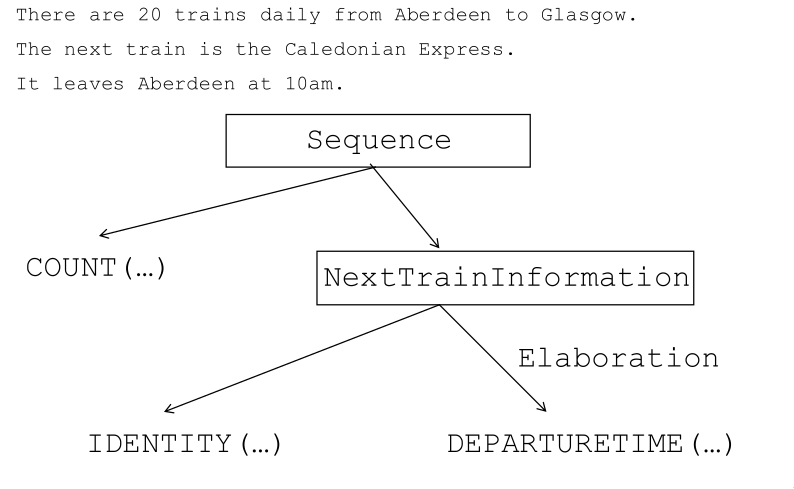
\includegraphics[scale=0.41]{03P/dp.png}
    \caption{I data owner possono fare hop out/hop in.}
\end{figure}

\paragraph{L'idea:}

\begin{itemize}
  \item Si studia l'effetto sulla query $q$ e sulla risposta di ogni singolo utente. 
  \item Quando si aggiunge un record vuol dire che una persona ha fatto \fancyglitter{hop in}. 
  \item Bisogna fare in modo che la risposta alla query sia leggermente randomizzata secondo una distribuzione di probabilità. Quindi se si fa due volte la stessa richiesta si riceveranno due risposte diverse vicine al valore esatto (fig: \ref{fig:lp}).
  \item Per impedire che una persona faccia molte query e ne faccia la media il rumore delle risposte a quella persona aumenta in base al numero di query.
  \item Assumiamo $\Omega$ come database e $Q$ come dominio di tutte le query.
  \item Il meccanismo randomizzato è $$\begin{aligned}
\mathcal{M}: \Omega \times Q &\to \mathcal{R} \\
(D, q) &\mapsto q\overline{(D)}
\end{aligned}$$
\end{itemize}

\begin{figure}[h]
    \centering
    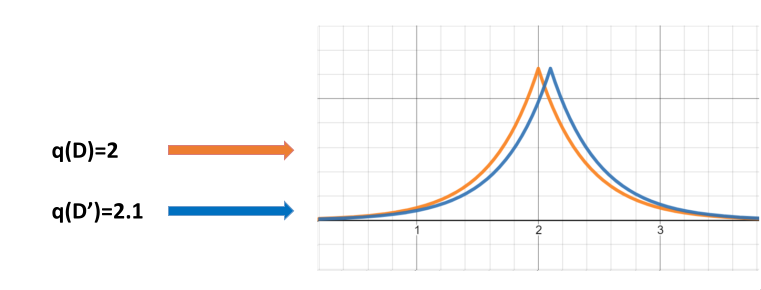
\includegraphics[scale=0.41]{03P/laplace.png}
    \caption{Distribuzione di Laplace.}
    \label{fig:lp}
\end{figure}

\nt{Si preferisce Laplace a Gauss perché discende molto velocemente.}

\dfn{$\epsilon$-Differential Privacy}{
  Un meccanismo $\mathcal{M}: \Omega \times Q \to  \mathcal{R}$ preserva la $\epsilon$-differential privacy, con $\epsilon > 0$ se, per qualsiasi query $q$ ogni datasets adiacenti $D, D' \in \Omega$ e ogni $r \in \mathcal{R}$: 
  $$e^{-\varepsilon} \leq \frac{\mathbb{P}(\mathcal{M}(q, D) = r)}{\mathbb{P}(\mathcal{M}(q, D') = r)} \leq e^{\varepsilon}$$
}

\nt{Minore è $\epsilon$ maggiore è la garanzia di privacy.}

\dfn{Meccanismo di Laplace}{
Dato un dataset $D$ è una query $q$ il meccanismo di Laplace restituisce im valore estratto da una distribuzione di Laplace $Lap(\mu, \sigma)$ centrata nel risultato vero $q(D)$.
$$\mathcal{M}_{\text{Lap}} : (D, q) \mapsto \text{Lap}\left(q(D), \frac{\text{GS}_1(q)}{\varepsilon}\right)$$ 

$$\mathcal{M}_{\text{Lap}} : (D, q) \mapsto q(D) + \text{Lap}\left(0, \frac{\text{GS}_1(q)}{\varepsilon}\right)$$

}

\cor{Global Sensitivity}{
  La global sensitivity è una misura di quanto è sensibile la variazione della risposta $q$ quando è calcolata su due datasets adiacenti 

  $$S_1(q) = \max_{D \sim D'} \|q(D) - q(D')\|_1$$
}

\thm{Meccanismo di Laplace}{
Il meccanismo di Laplace preserva la $\epsilon$-differential privacy.
}

\paragraph{Oltre il meccanismo di Laplace:}

\begin{itemize}
  \item Queries non numeriche: in questo caso non ha senso applicare una perturbazione numerica. 
  \item Differentially private selection: in alcuni casi anche un'aggiunta piccola può cambiare enormemente il risultato.
\end{itemize}

\dfn{Meccanismo Esponenziale}{
Consideriamo $R$ come l'insieme dei possibili output di una query $q$. $q$ restituisce il valore $r \in R$ che massimizza una funzione di utilità $U: \Omega \times R \to \bbR$.
}

\begin{figure}[h]
    \centering
    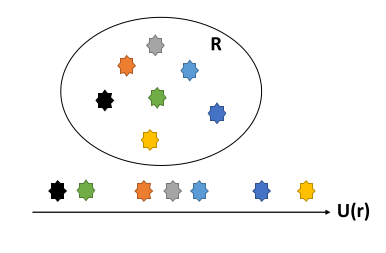
\includegraphics[scale=0.5]{03P/esp.png}
    \caption{Meccanismo esponenziale.}
\end{figure}

\thm{Post-processing}{
  Consideriamo $\mathcal{M}: \Omega \to \mathcal{R}$ come meccanismo di preservazione della $\epsilon$-differential privacy e $f$ come funzione con dominio $\mathcal{R}$. Allora $f \circ \mathcal{M}$ preserva la $\epsilon$-differential privacy.
}

\begin{figure}[h]
    \centering
    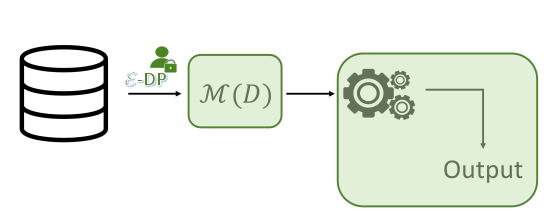
\includegraphics[scale=0.41]{03P/pp.png}
    \caption{Teorema di post-processing.}
\end{figure}

\thm{Composizione}{
  Consideriamo $\mathcal{M}_1: \Omega \to \mathcal{R}$ e  $\mathcal{M}_2: \Omega \to \mathcal{S}$ come meccanismi di preservazione della $\epsilon_{1,2}$-differential privacy. Allora il meccanismo $\mathcal{N}: \Omega \to \mathcal{R} \times \mathcal{S}$ tale che $\mathcal{N}(D) = (\mathcal{M}_1(D), \mathcal{M}_2(D))$ preserva sia la privacy di $\epsilon_1$ che di $\epsilon_2$.
} 

\begin{figure}[h]
    \centering
    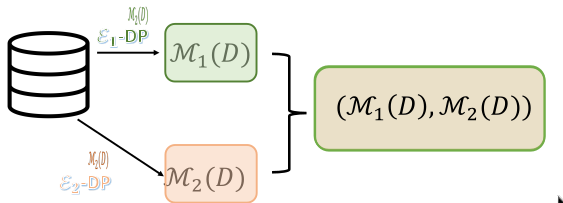
\includegraphics[scale=0.41]{03P/comp.png}
    \caption{Teorema di composizione.}
\end{figure}

\thm{Composizione Parallela}{
  Consideriamo $D \in \Omega$ come dataset e $\mathcal{M}: \Omega \to \mathcal{R}$ come meccanismo di preservazione della $\epsilon$-differential privacy, inoltre $D_1 \cup D_2$ formano un partizionamento di $D$. Il meccanismo $\mathcal{N}: \omega \to \mathcal{R} \times \mathcal{R}$ tale che $\mathcal{N}(D) = (\mathcal{M}(D_1), \mathcal{M}(D_2))$ soddisfa la $\epsilon$-differential privacy.

}

\begin{figure}[h]
    \centering
    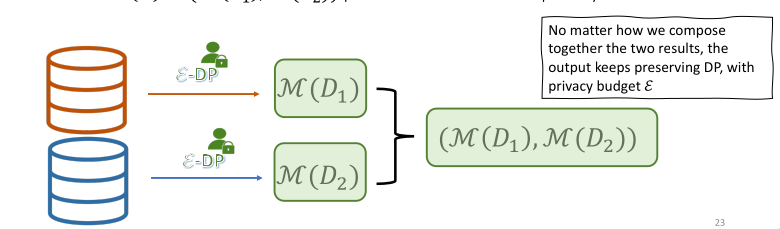
\includegraphics[scale=0.41]{03P/pc.png}
    \caption{Teorema di composizione parallela.}
\end{figure}

\dfn{($\epsilon, \delta$)-Differential Privacy}{
  Versione rilassata dell'$\epsilon$-differential privacy in cui è aggiunto un valore di tolleranza $\delta \in (0, 1)$. 
}

\paragraph{Caratteristiche:}

\begin{itemize}
  \item $\delta$ rappresenta una \fancyglitter{probabilità di fallimento} del meccanismo. 
  \item I teoremi appena visti continuano a valere. 
  \item Quando $\delta = 0$ coincide con la $\epsilon$-differential privacy. 
  \item Questo meccanismo è più debole dell'$\epsilon$-differential privacy: si ammettono fallimenti e la privacy non può essere preservata in alcuni casi.
\end{itemize}

\nt{Esistono ulteriori meccanismi che utilizzano la funzione gaussiana (funziona meglio con $\epsilon$ grande).}

\section{Privacy in Sistemi Distribuiti}

L'approccio tradizionale all'analisi dei dati da fonti distribuite è quello di raccogliere i dati una data warehouse centrale. Questo causa problemi di performance e connettività.

\paragraph{Analisi dei dati distribuiti:}

\begin{itemize}
  \item Semplicemente creare un algoritmo di ML non funziona. 
  \item I problemi relativi alla data warehouse persistono. 
\end{itemize}

\paragraph{A chi interessa quest'analisi?}

\begin{itemize}
  \item Governo e agenzie pubbliche. 
  \item Multinazionali. 
  \item Industrie. 
\end{itemize}

\paragraph{Classi di soluzione:}

\begin{itemize}
  \item \fancyglitter{Data obfuscation:} nessuno vede i dati reali. 
  \item \fancyglitter{Sommarizzazione:} solo i fatti necessari sono esposti. 
  \item \fancyglitter{Data separation:} 
    \begin{itemize}
      \item Solo parti fidate vedono i dati. 
      \item Approcci:
        \begin{itemize}
          \item I dati sono tenuti dai possessori o dai creatori. 
          \item Rilasci minimi. 
          \item Operazioni e analisi fatte da parti fidate. 
        \end{itemize}
      \item Problemi: 
        \begin{itemize}
          \item La parte fidata è desiderosa di fare le analisi? 
          \item I risultati delle analisi possono rivelare informazioni private?
        \end{itemize}
      \item Soluzioni:
        \begin{itemize}
          \item Secure Multiparty Computation. 
          \item Federate learning.
        \end{itemize}
    \end{itemize}
\end{itemize}

\dfn{Secure Multiparty Computation}{
  L'obiettivo è calcolare una funzione quando ogni parte ha qualche input.
}

\cor{1-out-2 Oblivious Transfer}{
  Prende in considerazioni due parti, il sender e il receiver. Il sender ha in input una coppia (x0, x1) e il receiver ha in input un bit $\sigma \in {0, 1}$ che specifica quale input è in grado di leggere. 
}

\nt{Il protocollo è strutturato in modo che il receiver impara $x_\sigma$ e niente altro e il sender non impara nulla.}

\begin{figure}[h]
    \centering
    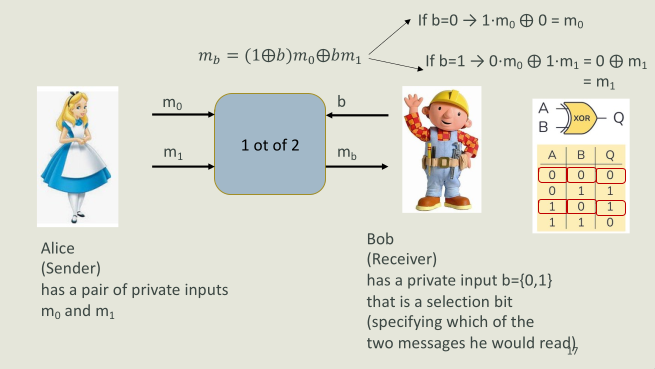
\includegraphics[scale=0.41]{03P/ab.png}
    \caption{Esempio classico.}
\end{figure}

\paragraph{Sicurezza del protocollo:}

\begin{itemize}
  \item Per il sender: un receiver corrotto non impara informazioni addizionali diverse dal messaggio che ha dichiarato di voler leggere. 
  \item Per il receiver: un sender corrotto non impara nulla sul receiver.
\end{itemize}

\paragraph{ID3 Algorithm:}

\begin{enumerate}
  \item Calcolo del guadagno di informazione per ogni feature. 
  \item Se tutte le righe non appartengono alla stessa classe splitta il dataset in sottoinsiemi usando la feature con minima entropia. 
  \item Crea un \fancyglitter{decision tree node} con la feature con minore entropia. 
  \item Se tutte le righe appartengono alla stessa classe rendi il nodo corrente una foglia con la classe come sua label. 
  \item Ripeti per le rimanenti features o finché il decision tree ha solo nodi foglia.
\end{enumerate}

\paragraph{Altri approcci complementari:}

\begin{itemize}
  \item Crittografia funzionale: 
    \begin{itemize}
      \item Generalizzazione della crittografia a chiave pubblica. 
    \end{itemize}
  \item Crittografia omomorfica: 
    \begin{itemize}
      \item Forma di crittografia che permette di effettuare calcoli su dati criptati senza decriptarli. 
      \item I risultati sono contenuti in forma criptata.
    \end{itemize}
  \item Federated learning: 
    \begin{itemize}
      \item Consente di allenare un algoritmo su molti dispositivi-vertici decentralizzati senza effettuare scambi.
    \end{itemize}
\end{itemize}


